\chapter{Marco de referencia}

\section{Marco Conceptual}
\label{sec:marco-conceptual}

El ajuste dinámico de frecuencia y voltaje parte de la relación entre el punto
de operación del hardware, la potencia consumida y el tiempo de ejecución. El
efecto de modificar ese punto depende del comportamiento de la carga, por lo
que resulta necesario establecer qué limita su desempeño y qué señales
permiten reconocer esa condición durante la ejecución. A partir de esta
relación se organiza el marco conceptual, comenzando por el modelo Roofline y
la caracterización de los regímenes \textit{compute-bound} y
\textit{memory-bound}, para continuar con la telemetría disponible en CPU y
GPU, los modelos ligeros utilizados para inferir ese comportamiento y los
mecanismos de control DVFS. Finalmente, se introduce el Producto
Energía--Retardo como referencia para relacionar el ahorro energético con el
efecto que una decisión de frecuencia produce sobre el tiempo de ejecución.

\subsection{Potencia CMOS y fundamento de DVFS}
\label{sec:marco-cmos}

La potencia consumida por un circuito CMOS incluye una componente estática,
asociada principalmente a corrientes de fuga, y una componente dinámica
producida por la conmutación de cargas capacitivas. Dado que DVFS modifica la
frecuencia y, según el estado operativo, también el voltaje de alimentación,
su efecto se relaciona de forma directa con la potencia dinámica, que puede
aproximarse como:

\begin{equation}
P_{\text{dyn}} = \alpha \cdot C \cdot V^{2} \cdot f
\end{equation}

donde $\alpha$ representa el factor de actividad, $C$ la capacitancia efectiva
conmutada, $V$ el voltaje de alimentación y $f$ la frecuencia de operación
\cite{Gonzalez1997}. La dependencia cuadrática respecto al voltaje explica por
qué una reducción del punto operativo puede disminuir de forma apreciable la
potencia, aunque ese beneficio no puede evaluarse sin considerar el tiempo de
ejecución. Una carga que pierde rendimiento al reducir la frecuencia puede
permanecer activa durante más tiempo y compensar parte del ahorro obtenido.
Esta relación física da origen al compromiso energía--rendimiento que debe
resolver una política DVFS.

\subsection{Modelo Roofline y regímenes de ejecución}
\label{sec:roofline}

El efecto de variar la frecuencia no es uniforme porque el rendimiento de una
carga puede estar condicionado por recursos distintos. El modelo Roofline
formaliza esta diferencia al relacionar la intensidad operacional con los
límites de cómputo y ancho de banda de memoria de la plataforma
\cite{Williams2009}. Su formulación básica es:

\begin{equation}
P = \min\left(P_{\text{pico}},\; I \cdot BW_{\text{pico}}\right)
\label{eq:roofline}
\end{equation}

donde $P_{\text{pico}}$ corresponde al rendimiento aritmético pico, $I$ a la
intensidad operacional y $BW_{\text{pico}}$ al ancho de banda pico de memoria.
Cuando el límite viene dado por $I \cdot BW_{\text{pico}}$, aumentar la
capacidad de cómputo no elimina la restricción impuesta por el movimiento de
datos y la carga se considera \textit{memory-bound}. Cuando el límite
corresponde a $P_{\text{pico}}$, el rendimiento queda ligado a la capacidad
aritmética y el régimen se considera \textit{compute-bound}.

\begin{figure}[H]
    \centering
    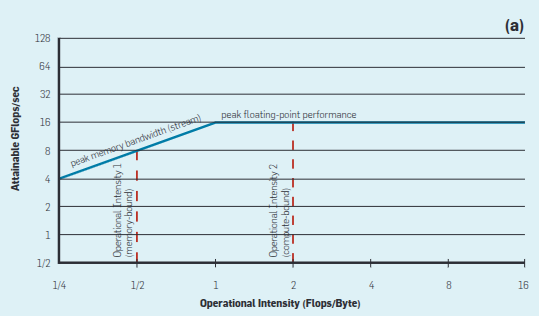
\includegraphics[width=0.72\textwidth]
        {figuras/fig_modelo_roofline_conceptual_williams2009.png}
    \caption[Modelo Roofline conceptual]{Modelo Roofline conceptual y relación
    entre el techo de ancho de banda de memoria y el techo de rendimiento de
    cómputo. Tomado de Williams et al. \cite[Fig.~1(a)]{Williams2009}.}
    \label{fig:modelo-roofline-conceptual}
\end{figure}

La separación entre ambos regímenes se encuentra en el \textit{ridge point},
obtenido al igualar las dos ramas del modelo:

\begin{equation}
I_{\text{ridge}} =
\frac{P_{\text{pico}}}{BW_{\text{pico}}}
\label{eq:ridge}
\end{equation}

Una intensidad inferior a $I_{\text{ridge}}$ sitúa la carga en la región
limitada por memoria y una intensidad superior en la región limitada por
cómputo \cite{Williams2009}. Este criterio es especialmente útil para el
proyecto porque permite construir una etiqueta a partir de una referencia
física del hardware, en lugar de asumir el régimen por el nombre del kernel o
por su comportamiento esperado. El punto de inflexión tampoco debe tratarse
como una constante universal. El techo de cómputo depende de la precisión
aritmética y puede variar con la frecuencia, mientras que el ancho de banda
pertenece a otro dominio y no necesariamente cambia en la misma proporción
\cite{Guerreiro2019,Ali2023}. Por ello, la interpretación de una carga debe
mantenerse vinculada a los techos correspondientes a la plataforma y al punto
operativo evaluado.
\label{sec:marco-ridge}

La intensidad operacional observada durante un intervalo $i$ se calcula como:

\begin{equation}
I_i =
\frac{\text{FLOPs}_i}{B_i^{\text{DRAM}}}
\label{eq:intensidad}
\end{equation}

$\text{FLOPs}_i$ representa el trabajo aritmético realizado y
$B_i^{\text{DRAM}}$ los bytes transferidos hacia o desde memoria principal
durante el mismo intervalo \cite{Williams2009}. Esta correspondencia temporal
es necesaria para conservar el significado físico de la razón. En CPU, el
trabajo aritmético puede obtenerse mediante eventos de rendimiento y el
tráfico hacia DRAM mediante contadores del controlador de memoria. En GPU, la
obtención de ambas magnitudes requiere una instrumentación de mayor detalle
que la telemetría ligera disponible durante la ejecución. Esta diferencia
explica por qué la referencia Roofline y las señales usadas posteriormente
para inferir el régimen no proceden necesariamente de la misma fuente.
\label{sec:intensidad}

\subsection{Telemetría microarquitectónica e instrumentación}
\label{sec:marco-telemetria}

La clasificación en línea requiere señales que reflejen el comportamiento del
hardware sin reproducir directamente el cálculo de la etiqueta Roofline. En
CPU, estas señales se obtienen principalmente mediante las Unidades de
Monitorización de Rendimiento, o PMU, que registran eventos asociados a la
ejecución. Parte de los contadores se reserva para eventos frecuentes, como
ciclos e instrucciones retiradas, mientras que otros son programables y
permiten seleccionar eventos definidos por la microarquitectura
\cite{IntelSDM2026}. Esta organización ofrece flexibilidad, pero también
impone un límite al número de eventos que pueden observarse al mismo tiempo.

% Se conserva aquí la figura PMU del archivo reescrito.

Cuando la cantidad de eventos solicitados supera los contadores físicos
disponibles, Linux puede multiplexarlos y estimar los conteos a partir del
tiempo durante el cual cada evento estuvo habilitado y realmente activo
\cite{Liu2024}. La relación entre \textit{time running} y
\textit{time enabled} permite reconocer esa situación y valorar si la lectura
mantiene una cobertura suficiente \cite{Liu2024,LinuxPerfEventOpen2026}. El
problema no es únicamente que existan pocos contadores, sino que una señal
observada de forma intermitente puede representar mal una carga cuyo
comportamiento cambia durante los periodos no medidos. Esta limitación
condiciona qué eventos resultan adecuados para alimentar un clasificador que
pretende operar sobre ventanas de ejecución.

La información tampoco procede de un único dominio. Los contadores de núcleo
registran eventos ligados a la actividad de los procesadores lógicos y
permiten derivar señales como IPC, tasa de fallos de caché, MPKI o ciclos de
espera. Los eventos \textit{uncore}, en cambio, cubren recursos compartidos
del zócalo, entre ellos el controlador de memoria y las interconexiones
\cite{IntelUncore2021}. Esta diferencia permite observar el tráfico que
alcanza DRAM, pero hace que su alcance y granularidad no coincidan
necesariamente con los contadores de núcleo. Para calcular intensidad
operacional, el trabajo aritmético y los bytes de memoria deben agregarse
sobre límites temporales compatibles antes de aplicar el criterio Roofline.
\label{sec:uncore}
\label{sec:ventanas}

Las métricas derivadas de los eventos de núcleo cumplen una función distinta a
la etiqueta. Un IPC bajo puede estar asociado con esperas, dependencias o
presión de memoria, mientras que los fallos de caché y los ciclos con
solicitudes de memoria pendientes aportan señales adicionales sobre la forma
en que progresa la ejecución \cite{Gregg2020,IntelPerfmon2026}. Ninguna de
estas variables demuestra por sí sola que una carga sea
\textit{memory-bound}. En Hyperion se utilizan como observaciones a partir de
las cuales el clasificador intenta aproximar una clase definida de manera
independiente mediante Roofline. Mantener esta separación evita convertir un
indicador microarquitectónico en una verdad física que no representa por sí
mismo.
\label{sec:marco-metricas-eficiencia}

Linux expone estas mediciones mediante \texttt{perf\_event}, que permite
acceder desde espacio de usuario a eventos de la PMU sin manipular
directamente sus registros \cite{LinuxPerfEventOpen2026,Weaver2015}. Para la
energía de CPU, Intel RAPL proporciona contadores acumulativos asociados a
dominios disponibles en la plataforma, entre ellos \textit{Package} y, cuando
existe soporte, DRAM \cite{David2010,Thamm2025}. La diferencia entre dos
lecturas permite obtener la energía correspondiente a un intervalo, aunque
esta medición representa los dominios expuestos por RAPL y no el consumo
eléctrico completo del nodo.
\label{sec:perfevent}
\label{sec:rapl}

La observabilidad de GPU tiene otra granularidad. NVML ofrece desde espacio de
usuario métricas agregadas de utilización, actividad de memoria, potencia,
energía y frecuencias de operación \cite{NVML2026}. Son adecuadas para
seguimiento continuo porque no requieren instrumentar cada kernel, pero no
proporcionan directamente los FLOPs y bytes necesarios para reconstruir la
intensidad operacional. Nsight Compute, por el contrario, puede perfilar
kernels CUDA con métricas de mayor detalle y obtener información suficiente
para caracterizar su posición en Roofline \cite{Nsight2026}. Su costo de
perfilado, que puede incluir varias pasadas sobre un mismo kernel, hace que su
papel sea distinto. \texttt{ncu} proporciona la referencia fuera de línea y
NVML las señales disponibles durante la inferencia, una separación que
mantiene la verdad de entrenamiento independiente de los proxies utilizados
por el modelo.
\label{sec:marco-nvml-ncu}
\label{sec:marco-interfaces}

\subsection{Control DVFS desde espacio de usuario}
\label{sec:marco-espacios-ejecucion}
\label{sec:dvfs-cpu}

El agente opera en espacio de usuario, mientras que el acceso directo a los
mecanismos del hardware permanece bajo control del kernel y de los
controladores del dispositivo \cite{Kerrisk2010,McCarty2015}. Esta separación
evita incorporar la lógica del proyecto como un módulo del kernel y permite
trabajar sobre interfaces estándar del sistema, aunque cada lectura,
inferencia y solicitud de frecuencia añade tiempo al lazo de decisión. La
utilidad del control depende, por tanto, de que ese costo sea pequeño frente a
la duración del comportamiento que se intenta aprovechar.

En CPU, Linux organiza la gestión de frecuencia mediante CPUFreq y los
mecanismos soportados por el procesador. Los \textit{governors} determinan
cómo se solicita un nivel de rendimiento, mientras que el controlador traduce
esa petición al hardware \cite{Hebbar2022,LinuxCPUFreq2026}. El
\textit{governor} \texttt{userspace}, cuando está disponible, permite que una
política externa participe en esa decisión, y las interfaces de CPUFreq
también exponen límites sobre los que puede actuar un servicio en espacio de
usuario. Hyperion se apoya en estas interfaces de control y se compara con
políticas nativas de referencia. \texttt{performance} mantiene una orientación
hacia niveles altos de rendimiento, \texttt{ondemand} responde a la carga
observada y \texttt{schedutil} incorpora información del planificador en la
selección de frecuencia \cite{Hebbar2022,LinuxCPUFreq2026}.

Una solicitud de frecuencia no equivale necesariamente al reloj que termina
usando el procesador. Mecanismos como \texttt{intel\_pstate}, HWP o Turbo
Boost pueden intervenir en el punto operativo efectivo según las condiciones
de ejecución \cite{LinuxIntelPstate2026,Hebbar2022}. Esta diferencia obliga a
distinguir entre la acción solicitada y el estado alcanzado, ya que la
comparación energética solo tiene sentido si el cambio atribuido a DVFS
ocurrió realmente. El mismo principio aplica al tiempo de transición. Una
decisión cuyo efecto tarda en materializarse puede perder utilidad cuando la
fase de la carga cambia antes de que el nuevo nivel llegue a aprovecharse.

En GPU, la relación entre frecuencia y rendimiento también depende del recurso
dominante. El dominio de procesamiento asociado a los SM y el dominio de
memoria no responden de la misma manera ante una variación del reloj
\cite{Guerreiro2019,Ali2023}. Una carga \textit{compute-bound} suele mostrar
mayor sensibilidad a la capacidad de procesamiento, mientras que en una carga
\textit{memory-bound} elevar el reloj de los SM puede aportar una mejora menor
si el movimiento de datos sigue imponiendo el límite. El régimen inferido
adquiere sentido para el control precisamente porque anticipa esa sensibilidad
y permite evitar cambios que añaden consumo sin una reducción proporcional
del tiempo.
\label{sec:dvfs-gpu}
\label{sec:dominios}

% Se conserva aquí la figura de dominios GPU del archivo reescrito.

El cambio de reloj en el acelerador tampoco es instantáneo. Entre la solicitud
y la estabilización del nuevo punto operativo existe una latencia que depende
del dispositivo y de la transición realizada \cite{Velicka2025}. Si ese
tiempo es comparable con la duración de la fase sobre la que se pretende
actuar, el beneficio potencial se reduce porque parte del intervalo transcurre
antes de alcanzar el estado deseado. La actuación DVFS en GPU debe
interpretarse, por ello, junto con la escala temporal de las fases y no
únicamente a partir de la clase inferida.

\subsection{Cargas de trabajo y calibración}
\label{sec:marco-cargas}

Las aplicaciones HPC combinan regiones con demandas diferentes sobre cómputo
y memoria, de modo que una medida agregada de toda la ejecución puede ocultar
cambios internos de comportamiento. Los kernels permiten aislar unidades de
trabajo con un patrón computacional definido, mientras que los benchmarks
aportan implementaciones reproducibles con diversidad algorítmica suficiente
para observar cómo responde la plataforma \cite{Williams2009,Gregg2020}. Su
procedencia no determina la clase. Una carga se considera
\textit{compute-bound} o \textit{memory-bound} a partir de la intensidad
operacional medida respecto al \textit{ridge point}, no porque la literatura
o el nombre del benchmark la describan de esa manera.

Los microbenchmarks cumplen una función distinta. Al reducir la ejecución a
operaciones controladas, permiten estimar propiedades de la plataforma como el
ancho de banda de memoria y el rendimiento aritmético \cite{Gregg2020}. Estas
mediciones sirven para construir los techos de Roofline y calibrar la
referencia con la que luego se etiquetan las cargas de caracterización. El
conjunto de entrenamiento se apoya así en benchmarks diversos, mientras que
los microbenchmarks proporcionan los límites físicos con los que se interpreta
su comportamiento.

\subsection{Clasificación supervisada ligera}
\label{sec:marco-ml-ligero}

La inferencia del régimen se plantea como un problema de clasificación
supervisada en el que una etiqueta conocida durante el entrenamiento se
relaciona con señales que también puedan observarse durante la operación del
sistema \cite{James2021}. En este caso, la etiqueta procede de Roofline y las
entradas corresponden a telemetría de bajo costo. La intensidad operacional y
las magnitudes que revelan directamente la regla utilizada para construir esa
etiqueta deben permanecer fuera del vector de características, pues incluirlas
convertiría la clasificación en una repetición del criterio de etiquetado y no
en una inferencia útil para el lazo de control.

El carácter ligero del modelo se define por su costo de operación y no por el
nombre del algoritmo. La regresión logística ofrece una referencia lineal,
mientras que los árboles de decisión representan relaciones no lineales
mediante reglas de partición sencillas \cite{James2021}. Random Forest y Extra
Trees combinan múltiples árboles para reducir la dependencia de una sola
partición, a cambio de evaluar varios estimadores durante la inferencia
\cite{Breiman2001,Geurts2006}. XGBoost construye el ensamble de forma
secuencial y permite representar interacciones más complejas entre
características \cite{Chen2016}. Comparar estas familias permite determinar si
el aumento de capacidad predictiva justifica también el costo temporal que
introduce en una decisión en línea.
\label{sec:marco-familias-modelos}

La evaluación debe reflejar tanto el desempeño global como el comportamiento
sobre cada clase. La matriz de confusión permite observar cómo se distribuyen
los errores entre \textit{compute-bound} y \textit{memory-bound}, mientras que
el $F_1$ combina precisión y sensibilidad y su promedio macro otorga el mismo
peso a ambas clases \cite{SokolovaLapalme2009}. Esta propiedad resulta útil
cuando la distribución de etiquetas no es uniforme, ya que evita que la clase
más frecuente determine por sí sola la lectura del resultado. Una línea base
mayoritaria proporciona además una referencia mínima para comprobar si las
señales de entrada contienen información discriminativa bajo el protocolo de
evaluación.
\label{sec:marco-evaluacion-clasificador}
\label{sec:marco-lineas-base}

La latencia de inferencia forma parte de esa evaluación porque cada predicción
consume tiempo dentro del ciclo de control. Un valor medio puede ocultar
ejecuciones ocasionalmente más lentas, por lo que percentiles como p95 y p99
permiten describir la cola de la distribución sin presentarla como un peor
caso absoluto \cite{Georges2007}. La elección de un modelo no puede separarse
por completo de este costo. Una mejora predictiva deja de ser atractiva si la
inferencia consume una fracción significativa del intervalo en el que todavía
puede aplicarse la decisión.
\label{sec:marco-costo-inferencia}

\subsection{Optimización de hiperparámetros y Optuna}
\label{sec:marco-optuna}

Además de los parámetros aprendidos durante el entrenamiento, cada familia de
modelos contiene hiperparámetros que condicionan su estructura o su proceso de
ajuste. La profundidad de un árbol, el número de estimadores de un ensamble o
la intensidad de regularización son ejemplos de valores que deben
seleccionarse antes de obtener el modelo final \cite{Bergstra2012}. Su
elección modifica tanto la capacidad de ajuste como la complejidad resultante,
de modo que comparar algoritmos sin considerar sus configuraciones puede
confundir las propiedades de una familia con una elección particular de
hiperparámetros.

Optuna organiza esta búsqueda mediante ensayos sucesivos o \textit{trials},
donde cada configuración se evalúa a partir de una función objetivo y los
resultados obtenidos orientan las propuestas posteriores \cite{Akiba2019}.
Entre los métodos disponibles se encuentra el \textit{Tree-structured Parzen
Estimator}, que utiliza los ensayos ya observados para modelar regiones
asociadas con mejores y peores resultados y concentrar parte de la exploración
donde existe mayor expectativa de mejora. La finalidad no es recorrer de forma
exhaustiva todas las combinaciones, sino asignar el presupuesto de evaluación
de manera más informada.

La optimización introduce, al mismo tiempo, un riesgo de adaptación a los
datos usados para escoger la configuración. Cuando la misma información
participa en la selección y en la estimación final del desempeño, la
evaluación puede quedar favorecida por el propio proceso de búsqueda. La
validación anidada separa ambas funciones mediante un nivel interno para
ajustar hiperparámetros y otro externo para estimar generalización
\cite{Cawley2010}. Si varias observaciones proceden de una misma familia
algorítmica, esa relación también debe preservarse durante la partición para
evitar que variantes estrechamente relacionadas aparezcan a ambos lados de la
evaluación \cite{Roberts2017}.

Esta separación estadística no corrige una fuga presente en las
características. Una variable derivada de la etiqueta, o suficientemente
cercana a la regla que la construye, puede ofrecer al modelo información que
no estaría disponible en una predicción real \cite{Kaufman2012}. En una
clasificación basada en Roofline, la distinción entre la fuente de verdad y la
fuente de inferencia debe mantenerse desde el diseño del conjunto de datos.
Optuna puede encontrar una configuración eficiente dentro del espacio
propuesto, pero no puede convertir en válida una entrada que ya contiene la
respuesta que el modelo intenta aprender.

\subsection{Producto Energía--Retardo}
\label{sec:marco-edp}

La reducción de potencia no implica necesariamente una mejora energética si el
tiempo de ejecución aumenta en una proporción suficiente para compensarla. Por
esta razón, la evaluación de DVFS requiere observar ambas magnitudes de forma
conjunta. El Producto Energía--Retardo, o EDP, expresa este compromiso mediante
\cite{Laros2013}:

\begin{equation}
EDP = E \cdot T
\end{equation}

$E$ representa la energía consumida y $T$ el tiempo de ejecución. Un valor
menor indica un compromiso más favorable bajo este criterio, pero la
formulación puede modificarse cuando se desea penalizar con mayor fuerza la
degradación temporal:

\begin{equation}
\mathrm{ED}^{n}\mathrm{P} = E \cdot T^{n}
\label{eq:ednp}
\end{equation}

Con $n=1$ se recupera el EDP clásico y con $n=2$ se obtiene ED$^{2}$P, donde
el tiempo adquiere mayor peso \cite{Laros2013,Ali2023}. La elección del
exponente modifica la forma en que se ordenan las configuraciones y debe
mantenerse explícita al comparar políticas. Para Hyperion, esta familia de
métricas permite valorar si una reducción energética justifica el cambio de
tiempo producido por la actuación DVFS, evitando interpretar potencia, energía
o rendimiento de manera aislada.

\section{Estado del Arte}
\label{sec:estado-del-arte}

La gestión energética en sistemas de alto rendimiento ha pasado de aplicar
reducciones de frecuencia de forma relativamente uniforme a considerar con
mayor detalle el comportamiento de cada carga. Este cambio responde a una
limitación conocida de DVFS. Reducir el punto operativo puede disminuir la
potencia, pero el resultado energético depende de cuánto se prolongue la
ejecución. Los trabajos más próximos a esta investigación pueden leerse, por
tanto, como una evolución desde la caracterización de esa sensibilidad hasta
mecanismos capaces de reconocer fases y actuar durante la ejecución.

Calore et al. \cite{Calore2017} analizaron el efecto de DVFS sobre una CPU
Intel Haswell y una GPU NVIDIA K80 utilizando kernels y una aplicación HPC
completa. Al modificar la frecuencia en regiones de ejecución observaron que
una misma configuración no ofrece el mismo compromiso entre energía y tiempo
para toda la aplicación. El trabajo establece una relación directa entre el
comportamiento local de la carga y la conveniencia de cambiar el punto
operativo, aunque la actuación depende de conocer previamente las regiones
donde debe aplicarse. El problema queda entonces planteado de una forma que
resulta relevante para Hyperion. Si las fases responden de manera distinta a
DVFS, el control necesita reconocer esas diferencias sin depender de
anotaciones específicas en cada aplicación.

Guerreiro et al. \cite{Guerreiro2019} abordaron esa necesidad desde la
caracterización de aplicaciones GPGPU. Su propuesta recoge métricas en una
configuración inicial y utiliza esa información para estimar cómo responderá
la carga ante otros estados de frecuencia de cómputo y memoria. Con ello
reducen la necesidad de recorrer exhaustivamente el espacio DVFS y muestran
que la sensibilidad de una aplicación puede anticiparse a partir de señales
del hardware. El enfoque, sin embargo, se concentra en caracterizar la
respuesta de una carga y no en seguir de manera continua las transiciones
entre fases \textit{compute-bound} y \textit{memory-bound}.

Ali et al. \cite{Ali2023} avanzaron en una dirección similar mediante modelos
de potencia y tiempo construidos a partir de métricas obtenidas en la
configuración predeterminada de la GPU. A partir de esas estimaciones
seleccionan frecuencias sin ejecutar cada alternativa y consideran de forma
conjunta el ahorro energético y la degradación del desempeño. En las
plataformas evaluadas reportaron reducciones promedio de energía de 29.6\% en
NVIDIA GA100 y 22.6\% en GV100, con pérdidas de rendimiento de 5.2\% y 4.7\%,
respectivamente. El resultado refuerza la idea de que una caracterización
limitada puede ser suficiente para orientar la selección de frecuencia, aunque
nuevamente la unidad de decisión es la carga caracterizada y no una sucesión
de fases detectadas durante la ejecución.

La identificación automática del régimen aparece de manera más directa en
MCBound, propuesto por Antici et al. \cite{Antici2024}. El trabajo formula la
separación entre cargas \textit{memory-bound} y \textit{compute-bound} como un
problema de clasificación a partir de datos de ejecuciones HPC. Sobre
información del supercomputador Fugaku, los autores reportaron un $F_1$ macro
de al menos 0.89, lo que muestra que el régimen puede inferirse mediante
señales observables sin depender exclusivamente de una clasificación manual.
MCBound se aproxima al problema predictivo de Hyperion, pero utiliza la clase
para caracterizar trabajos y no como entrada directa de una política que
modifique la frecuencia de CPU o GPU durante la ejecución.

Simsek et al. \cite{Simsek2024} estudiaron precisamente la actuación por
regiones en simulaciones astrofísicas ejecutadas sobre GPU. La instrumentación
de SPH-EXA les permitió modificar la frecuencia en puntos determinados y
reducir el consumo energético por GPU hasta en 7.82\%, con una degradación de
rendimiento cercana a 2.95\%. El resultado confirma que adaptar la frecuencia
dentro de una misma aplicación puede ser más conveniente que mantener un
estado uniforme, aunque la política continúa ligada a regiones conocidas del
código. La diferencia frente a una estrategia basada en telemetría es
importante, porque en esta última la frontera entre comportamientos debe
detectarse a partir de lo que el hardware expone durante la ejecución.

DRLCAP, presentado por Wang et al. \cite{Wang2024}, lleva esta idea hacia un
control \textit{online} basado en aprendizaje por refuerzo profundo. El marco
detecta cambios de fase y ajusta límites de frecuencia de GPU durante la
ejecución, con una reducción media de energía del 22\% y menos de 3\% de
degradación del rendimiento en las arquitecturas estudiadas. Este antecedente
demuestra que una política aprendida puede intervenir en tiempo real, pero
adopta una solución más compleja y centrada en GPU. Hyperion parte de otra
restricción. La inferencia debe mantenerse ligera y la política debe poder
operar sobre un entorno heterogéneo donde CPU y GPU no comparten las mismas
fuentes de telemetría ni los mismos mecanismos de actuación.

La literatura revisada cubre, por separado, los componentes principales del
problema. Calore et al. muestran que la respuesta a DVFS cambia entre regiones,
Guerreiro et al. y Ali et al. relacionan telemetría con sensibilidad y
selección de frecuencia, MCBound demuestra que el régimen puede inferirse
mediante clasificación y los trabajos de Simsek et al. y Wang et al. muestran
distintas formas de actuación durante la ejecución. La separación entre estas
contribuciones deja espacio para estudiar una integración donde la clase
inferida funcione como contexto de una política DVFS y donde el costo de
observar, clasificar y actuar forme parte de la evaluación.

Esta integración también exige tratar CPU y GPU como dispositivos distintos y
no como dos instancias del mismo problema. La mayoría de los trabajos recientes
de predicción y control se concentra en GPU, mientras que Calore et al. ofrecen
una de las referencias que consideran ambos tipos de dispositivo
\cite{Calore2017}. En CPU, las PMU y los contadores \textit{uncore} permiten
observar señales que no tienen un equivalente directo en NVML. En GPU, el
perfilado detallado necesario para construir la referencia Roofline tiene un
costo incompatible con la inferencia ligera y debe separarse de la telemetría
utilizada durante el control. El aporte que se investiga en Hyperion se sitúa
en esa diferencia de observabilidad, utilizando una referencia física común
para definir el régimen, pero aceptando que las señales con las que se intenta
inferirlo y los mecanismos de frecuencia disponibles son distintos en cada
dispositivo.